%%%%%%%%%%%%%%%%%%%%%%%%%%%%%%%%%%%%%%%%%
% Sullivan Business Report
% LaTeX Template
% Version 1.0 (May 5, 2022)
%
% This template originates from:
% https://www.LaTeXTemplates.com
%
% Author:
% Vel (vel@latextemplates.com)
%
% License:
% CC BY-NC-SA 4.0 (https://creativecommons.org/licenses/by-nc-sa/4.0/)
%
%%%%%%%%%%%%%%%%%%%%%%%%%%%%%%%%%%%%%%%%%

%----------------------------------------------------------------------------------------
%	CLASS, PACKAGES AND OTHER DOCUMENT CONFIGURATIONS
%----------------------------------------------------------------------------------------

\documentclass[
	a4paper, % Paper size, use either a4paper or letterpaper
	12pt, % Default font size, the template is designed to look good at 12pt so it's best not to change this
	%unnumberedsections, % Uncomment for no section numbering
]{persist}

\addbibresource{lit.bib} % BibLaTeX bibliography file

%----------------------------------------------------------------------------------------
%	REPORT INFORMATION
%----------------------------------------------------------------------------------------

\reporttitle{Performant Simulation of Inland Ship Traffic: PERIST} % The report title to appear on the title page and page headers, do not create manual new lines here as this will carry over to page headers

\reportsubtitle{A documentation for using the PERSIST framework to model and assess inland vessel traffic} % Report subtitle, include new lines if needed

\reportauthors{Niklas Paulig\\Fabian Hart\\Ostap Okhrin} % Report authors/group/department, include new lines if needed

\reportdate{\today} % Report date, include new lines for additional information if needed

\rightheadercontent{
\includegraphics[width=3cm]{tu.pdf}} % The content in the right header, you may want to add your own company logo or use your company/department name or leave this command empty for no right header content

%----------------------------------------------------------------------------------------

\begin{document}

%----------------------------------------------------------------------------------------
%	TITLE PAGE
%----------------------------------------------------------------------------------------

\thispagestyle{empty} % Suppress headers and footers on this page

\begin{fullwidth} % Use the whole page width
	\vspace*{-0.075\textheight} % Pull logo into the top margin
	
	\hfill
\includegraphics[width=5cm]{img/tu.pdf} % Company logo

	\vspace{0.15\textheight} % Vertical whitespace

	\parbox{0.9\fulltextwidth}{\fontsize{50pt}{52pt}\selectfont\raggedright\textbf{\reporttitle}\par} % Report title, intentionally at less than full width for nice wrapping. Adjust the width of the \parbox and the font size as needed for your title to look good.
	
	\vspace{0.03\textheight} % Vertical whitespace
	
	{\LARGE\textit{\textbf{\reportsubtitle}}\par} % Subtitle
	
	\vfill % Vertical whitespace
	
	{\Large\reportauthors\par} % Report authors, group or department
	
	\vfill\vfill\vfill % Vertical whitespace
	
	{\large\reportdate\par} % Report date
\end{fullwidth}

\newpage

%----------------------------------------------------------------------------------------
%	DISCLAIMER/COPYRIGHT PAGE
%----------------------------------------------------------------------------------------

\thispagestyle{empty} % Suppress headers and footers on this page

\begin{twothirdswidth} % Content in this environment to be at two-thirds of the whole page width
	\footnotesize % Reduce font size
	
	\subsection*{Disclaimer}

	This documentation is provided "as is" and to the best of our knowledge, contains accurate and reliable information. However, it is important to note that this documentation is a work in progress and may not be complete or up-to-date. We make no representations or warranties of any kind, express or implied, about the completeness, accuracy, reliability, suitability, or availability with respect to the documentation or the information contained within it. Any reliance you place on this documentation is therefore strictly at your own risk. We reserve the right to make changes to this documentation at any time without prior notice.
	
	\subsection*{Copyright}
	
	\textcopyright~[2023] [Technische Universtiät Dresden | Bundesanstalt für Wasserbau] 
	
	This work and its contents are protected under copyright laws. Unauthorized reproduction, distribution or use of this work, in whole or in part, is strictly prohibited and may result in severe civil and criminal penalties. Any unauthorized use or reproduction of this work will be pursued to the fullest extent of the law. This includes but is not limited to reproduction or distribution of the work in any form or by any means, including electronic or mechanical methods, without prior written permission from the copyright holder.

	For permission to use this work, please contact the publisher.
	
	\subsection*{Contact}
	
	Niklas Paulig\\
	Institut für Wirstschaft und Verkehr\\
	Würzburger Straße 35, 01187 Dresden
	
	Contact: niklas.paulig@tu-dresden.de
	
	\vfill % Push the following down to the bottom of the page
	
	\subsubsection*{Changelog}
	
	\scriptsize % Reduce font size further
	
	\begin{tabular}{@{} L{0.05\linewidth} L{0.15\linewidth} L{0.6\linewidth} @{}} % Column widths specified here, change as needed for your content
		\toprule
		v1.0.5 & 2023-03-06 & 
		PERSIST now offers a shell entry point and can be invoked directly as: \verb|$ persist -c path/to/config.toml|\\
		v1.0.4 & 2023-03-03 & Dependencies are now downloaded on install. Configuration file is now using the .toml format. Logger output, network weight files and river data now have configurable paths. Plotting modules are only imported if visualize = true in the configuration file. Added argument parser to invoke PERSIST via a python module call: python -m persist -c path/to/config.toml.\\
		v1.0.3 & 2022-08-24 & Vessels are now modeled individually by a class. All ships share the same river object. Drivable area per vessel is pre-computed for a discrete range of squat values. Ship draught mandatory in configuration file.\\
		v1.0.2 & 2033-06-23 & Bug fixes.\\
		v1.0.1 & 2022-06-20 & Enabled logging for the entire simulation process. The data of individual vessels will be logged into a separate file, located in the simlogs folder.\\
		\bottomrule
	\end{tabular}
\end{twothirdswidth}

\newpage

%----------------------------------------------------------------------------------------
%	TABLE OF CONTENTS
%----------------------------------------------------------------------------------------

\begin{twothirdswidth} % Content in this environment to be at two-thirds of the whole page width
	\tableofcontents % Output the table of contents, automatically generated from the section commands used in the document
\end{twothirdswidth}

\newpage

%----------------------------------------------------------------------------------------
%	SECTIONS
%----------------------------------------------------------------------------------------
\section{Introduction} 

\subsection{About PERSIST} % Top level section

Traffic modeling is an important component for the safety and economical development of inland waterways. It enables investigating system behavior and development under static and dynamic environmental conditions, such as decline in water levels, changing number of traffic participants or changing behavior of individuals.

As part of a research collaboration, a micro traffic simulation model (TSM) called Performant Simulation of Inland Ship Traffic (PERSIST) was developed. The model uses agents to control individual inland vessels, which were trained through a machine learning approach to select appropriate trajectories and make decisions on ship-ship interactions while considering hydraulic and traffic constraints. PERSIST provides an excellent foundation for advanced applications, including traffic forecasting and analysis related to shipping traffic automation. \sidenote{The mentioned applications are a non-exhaustive snapshot at the time of writing, as PERSIST is currently under development.}

In short, PERSIST allows you run a traffic simulation by specifying a configuration file, which contains all relevant information about the simulation scenario, such as the number of vessels, their starting positions, desired powers, masses, dimensions, and the waterway. The simulation is then run for a specified number of time steps, and the resulting trajectories are stored in a log file. The log file can then be used to analyze the simulation results.

\subsection{Structure of this documentation} % Second level section

This documentation is intended to provide a comprehensive overview of the PERSIST framework, and is therefore split into two parts. 

Part one serves as a Practitioner's Guide, providing a detailed instruction manual on how to install and use the PERSIST framework and its functions. We will explain the functionality of the most important modules and provide examples on how to use, and adapt them.\sidenote{Most code examples in this documentation are written in Python, so a basic understanding of the language is required.} We will take a look at the configuration files and explain how to set up a simulation scenario. Finally, we will provide a detailed description of the output visualizations and logs and how to interpret them.

Part two serves as a methodological reference, providing a detailed description of the underlying concepts and methods used in the PERSIST framework. We will explain the algorithmic foundation as well as the training and testing procedures for the machine learning models used in PERSIST.

\section{Practitioner's Guide}

\subsection{Installation}

\paragraph{Prerequisites}

PERSIST is written in Python 3.9 and due to the use of type hinting with built-in types it currently does not support backwards compatibility. You can install the latest version of Python from the official website via this \href{https://www.python.org/downloads/}{link} \ExternalLink.

After obtaining a working Python installation, you can obtain a copy of the PERSIST framework either from the official GitHub repository via this link... \ExternalLink or by downloading the latest release from the official website via this link... \ExternalLink.

After downloading and/or unpacking the PERSIST framework to a folder of your choice, we recommend installing it into a virtual environment.

\subsubsection{Setting up a virtual environment}

\begin{note}
	This section is optional. If you do not want to use a virtual environment, you can skip this section and proceed to the next section.
\end{note}

A virtual environment is a self-contained directory tree that contains a Python installation for a particular version of Python, plus a number of additional packages. Different virtual environments can use different Python versions and can have different sets of installed packages. This allows you to have multiple versions of Python and multiple versions of the same package installed on the same system without conflicts.

You can create a virtual environment by running the following command in your terminal:\sidenote{If not stated otherwise, all command-line instructions in this documentation are written for Linux-based systems. If you are using a Windows system, we recommend using the \href{https://docs.microsoft.com/en-us/windows/wsl/install-win10}{Windows Subsystem for Linux} \ExternalLink to run Linux commands.}

\begin{lstlisting}[language=bash]
	python -m venv .persist
\end{lstlisting}

This will create a new folder called \emph{.persist} in your current working directory. To activate the virtual environment, run the following command:

\begin{lstlisting}[language=bash]
	source .persist/bin/activate
\end{lstlisting}

You can deactivate the virtual environment at any time by running the following command:

\begin{lstlisting}[language=bash]
	deactivate
\end{lstlisting}

\subsubsection{Installing PERSIST}

After activating the virtual environment, make sure you are in the root directory of the PERSIST framework and run the following command:\sidenote{PERSISTs dependency management is handled via poetry. If you do not have poetry installed, you can install it by following the instructions on the official website via this \href{https://python-poetry.org/docs/\#installation}{link} \ExternalLink.}

\begin{lstlisting}[language=bash]
	pip install .
\end{lstlisting}

In case you want to install PERSIST in development mode, i.e. you do not have to reinstall the package after manual changes in the code, run the following command instead:

\begin{lstlisting}[language=bash]
	pip install -e .
\end{lstlisting}

To verify that the installation was successful, you can run:

\begin{lstlisting}[language=bash]
	persist 
\end{lstlisting}

which should print a welcome message together with the current version of PERSIST.

Congrationlations - you have successfully installed PERSIST!

\subsection{Configuration files}

\paragraph{Basic information}

To prepare and execute simulations, PERSIST uses two configuration files in the \verb|.toml|\sidenote{TOML (Tom's Obvious, Minimal Language) is a configuration file format designed to be easy to read and write, yet unambiguous and precise. It aims to be a minimal configuration file format that can be easily parsed and manipulated by both humans and machines.} file format. 

The first file, called \verb|rivers.toml| contains names and data paths of all rivers that are available for simulation. This file is always located under \verb|./data/rivers/rivers.toml| and should only be changed if you want to add or remove rivers from the simulation.

The second file will be the main configuration file of the simulation, and can be named arbitrarily, as long as it has the \verb|.toml| file extension. This file contains all relevant information about the simulation scenario, such as the number of vessels, their starting positions, desired powers, masses, dimensions, and the waterway specifications. This file has no specific location, although we recommend storing it in the \verb|./configs/| folder.

We will now explain the structure of both files in detail.

\subsubsection{rivers.toml}

As per release, the \verb|rivers.toml| file contains the following information:
\begin{lstlisting}
	[lower_rhine]
	path = "lr"

	[middle_rhine]
	path = "mr"
\end{lstlisting}

The name in brackets is the name of the river, which is used to reference the river in the main configuration file. The \verb|path| key contains the path to the river data folder, which is located in the \verb|./data/rivers/| folder. The path is relative to the \verb|./data/rivers/| folder, so in this case the \verb|lower_rhine| river data folder is located at \verb|./data/rivers/lr/|.

For information about adding new rivers to the simulation, please refer to the \emph{Adding new rivers} section.

\subsubsection{Main configuration file}

The main configuration file contains all relevant information about the simulation scenario. The following example shows the structure of the \verb|demo.toml| file which comes with the PERSIST framework:

\begin{lstlisting}
	[River]
	river_name = "lower_rhine"
	GPW = 26
	BPD = 20

	[Ships]
	lengths = [100, 100, 100, 100, 100, 100 ]
	widths = [10, 10, 10, 10, 10, 10 ]
	masses = [100_000, 100_000, 100_000, 100_000, 100_000, 100_000 ]
	draughts = [2.8, 2.8, 2.8, 2.8, 2.8, 2.8 ]
	x_locations = [17_900, 18_300, 18_800, 25_100, 25_600, 26_300 ]
	y_locations = [190, 190, 190, 310, 310, 310 ]
	overtaking_levels = [1, 1, 1, 1, 1, 2 ]
	directions = [ 1, 1, 1, -1, -1, -1 ]
	desired_powers = [ 700_000, 600_000, 300_000, 300_000, 600_000, 700_000 ]

	[Visualization]
	visualize = false
	freeze = true
	utm_transform = true
	followed_vessel = 5
	zoom = 1_500

	[Simulation]
	speed_up = 1
	n_iters = 2_000

	[Data]
	river_path = "data/rivers"
	onnx_path = "data/onnx_nets"
	logging_root = "simlogs"
\end{lstlisting}

The file is divided into several sections, each of which will be explained in detail. 

\paragraph{[River]}

The \verb|River| section contains information about the river that is to be simulated. The \verb|river_name| key contains the name of the river as specified in the \verb|rivers.toml| file. The \verb|GPW| and \verb|BPD| keys contain information about the grid specification used by the specified river file. 

\begin{marginfigure}
	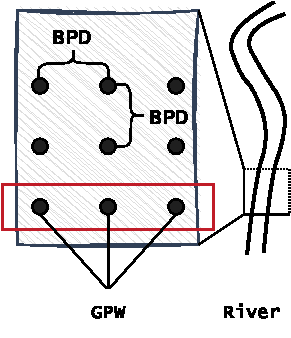
\includegraphics[width=\linewidth]{img/bpdgpw.pdf}
	\caption{GPW and BPD specification.}
	\label{fig:bpdgpw}
\end{marginfigure}

GPW (Grid Points per Width) specify how many grid points are used to discretize the width of the river. BPD (Base Point Distance) specifies the distance between two grid points in the horizontal and vertical irection (See Figure \ref{fig:bpdgpw} on the right). 

\begin{note}
	For the simulation to work, the GPW and BPD values must match the values used to generate the river data file. If you are using one of the rivers that come with the PERSIST framework, you do not need to change these values.
\end{note}

In our example we are using the \verb|lower_rhine| river, which has a GPW of 26 and a BPD of 20, meaning that the river is discretized into 26 grid points in the width direction, and that the distance between two grid points is 20 meters.

\paragraph{[Ships]}

The \verb|Ships| section contains information about the vessels that are to be simulated. The \verb|lengths|, \verb|widths|, \verb|masses|, and \verb|draughts| keys contain the lengths, widths, masses, and draughts of the vessels in meters, kilograms, and meters, respectively. 


The \verb|x_locations| and \verb|y_locations| keys contain the starting positions of the vessels in meters, given a flat projection of the river onto the x-y plane as seen in Figure \ref{fig:flatproj}.
\begin{marginfigure}
	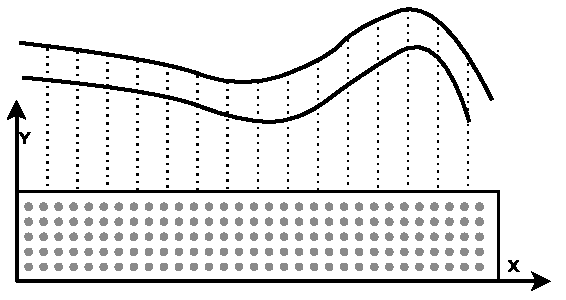
\includegraphics[width=\linewidth]{img/flatproj.pdf}
	\caption{Flat projection of the river onto the x-y plane.}
	\label{fig:flatproj}
\end{marginfigure}
In the flat projection, the river starts at the origin and flows downstream for increasing x values.


The \verb|overtaking_levels| key contains the overtaking levels of the vessels. A vessel can and will only overtake vessel with overtaking levels that are lower than its own. For example, a vessel with an overtaking level of 2 will overtake vessels with overtaking levels of 1 and 0, but not vessels with overtaking levels of 2 or higher. An overtaking level of 0 is equivalent to not overtaking at all.


The \verb|directions| key contains the directions in which the vessels are to be simulated. A value of 1 means that the vessel will advance downstream, and a value of -1 means that the vessel will advance upsteam. 


The \verb|desired_powers| key contains the desired powers of the vessels in watts. The maximum power of the vessel depends on the type of vessel simulated. Currently only a single vessel type (Europaschiff 100x10m) can be simulated, which has a maximum power of 1,000,000 watts. \sidenote{For future versions, this specification may be replaced by directly specifying the vessel type.}

\paragraph{[Visualization]}

The \verb|Visualization| section contains information about the visualization of the simulation. 

\begin{note}
	Due to its implementation in \emph{matplotlib}, the visualization module of PERSIST is very slow and thus intended to be a visual debugging tool only. Logging is  disabled when the visualization is enabled.
\end{note}

The \verb|visualize| key specifies whether the simulation should be visualized or not. 

The \verb|freeze| key specifies whether the simulation should be frozen at the beginning of the simulation. Freezing locks the camera at the average position of every vessel at the specified zoom level.\sidenote{This feature is experimental and may not work as intended. If you cannot see the vessels in the visualization, try changing the zoom level to a higher value.}

The \verb|utm_transform| key specifies whether the visualization should be transformed into the UTM coordinate system. If set to \verb|false|, the visualization will be in the flat projection as seen in Figure \ref{fig:flatproj}.

The \verb|followed_vessel| key specifies which vessel should be followed by the visualization. The first vessel has an index of 0, the second vessel has an index of 1, and so on. 

The \verb|zoom| key specifies the zoom level of the visualization in meters of radius around the followed vessel (see Figure \ref{fig:zoom}).
\begin{marginfigure}
	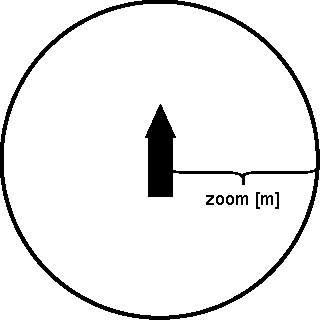
\includegraphics[width=\linewidth]{img/zoom.pdf}
	\caption{Visualization zoom level.}
	\label{fig:zoom}
\end{marginfigure}


\paragraph{[Simulation]}

The \verb|Simulation| section contains information about the simulation itself.

The \verb|speed_up| key specifies the speed up factor of the simulation. A value of 1 means that the positions of the vessels are updated once per second. A value of 2 means that the positions of the vessels are updated every two seconds, and so on.

The \verb|n_iters| key specifies the number of iterations that the simulation should run for.\sidenote{Currently, there is no option for the simulation to run in sandbox mode (indefinitely), as vessels leaving the river are not yet handled.}

\paragraph{[Data]}

The \verb|Data| section contains information about the storage folders of the simulation.

The \verb|river_path| key specifies the path to the river data folder. This is also where the \verb|rivers.toml| file must be located.

The \verb|onnx_path| key specifies the path to the exported neural network model. Unless you retrained the neural networks and saved them to a different location, you do not need to change this value.

The \verb|logging_root| key decides where all the logfiles of this configuration will be saved to. If the folder does not exist, it will be created. The logfiles will be saved in a subfolder named after the current date, time and number of vessels simulated. This will be discussed in more detail in Section ....

\subsection{Logging}

\paragraph{Text-based logging}

PERSIST features a comprehensive logging system for every stage of the simulation. Upon starting the simulation, a new folder will be created in the \verb|logging_root| folder specified in the configuration file. This folder will be named after the current date, time and number of vessels simulated. 
\begin{note}
	The logging folder will be named \verb|YYYY-MM-DD-HHMMSS_rivername_nvessels|
\end{note}

Inside this folder, a logfile will be created for every vessel simulated. The logfile contains information about the position, speed, power, and overtaking level of the vessel at each time step. The logfiles are saved in the \verb|csv| format, which can be opened in any spreadsheet software such as Microsoft Excel or LibreOffice Calc.

Additionally to the vessel logfiles, a copy of the configuration file, and all print outs to \verb|stdout| (saved in \verb|run.log|) will be saved in the logging folder. 

\paragraph{Graphical logging}

For every completed simulation, PERSIST will generate a summary graph of the simulation. This graph contains a visual representation of the speeds, locations and overtaking levels of all vessels over the course of the simulation.
\begin{marginfigure}
	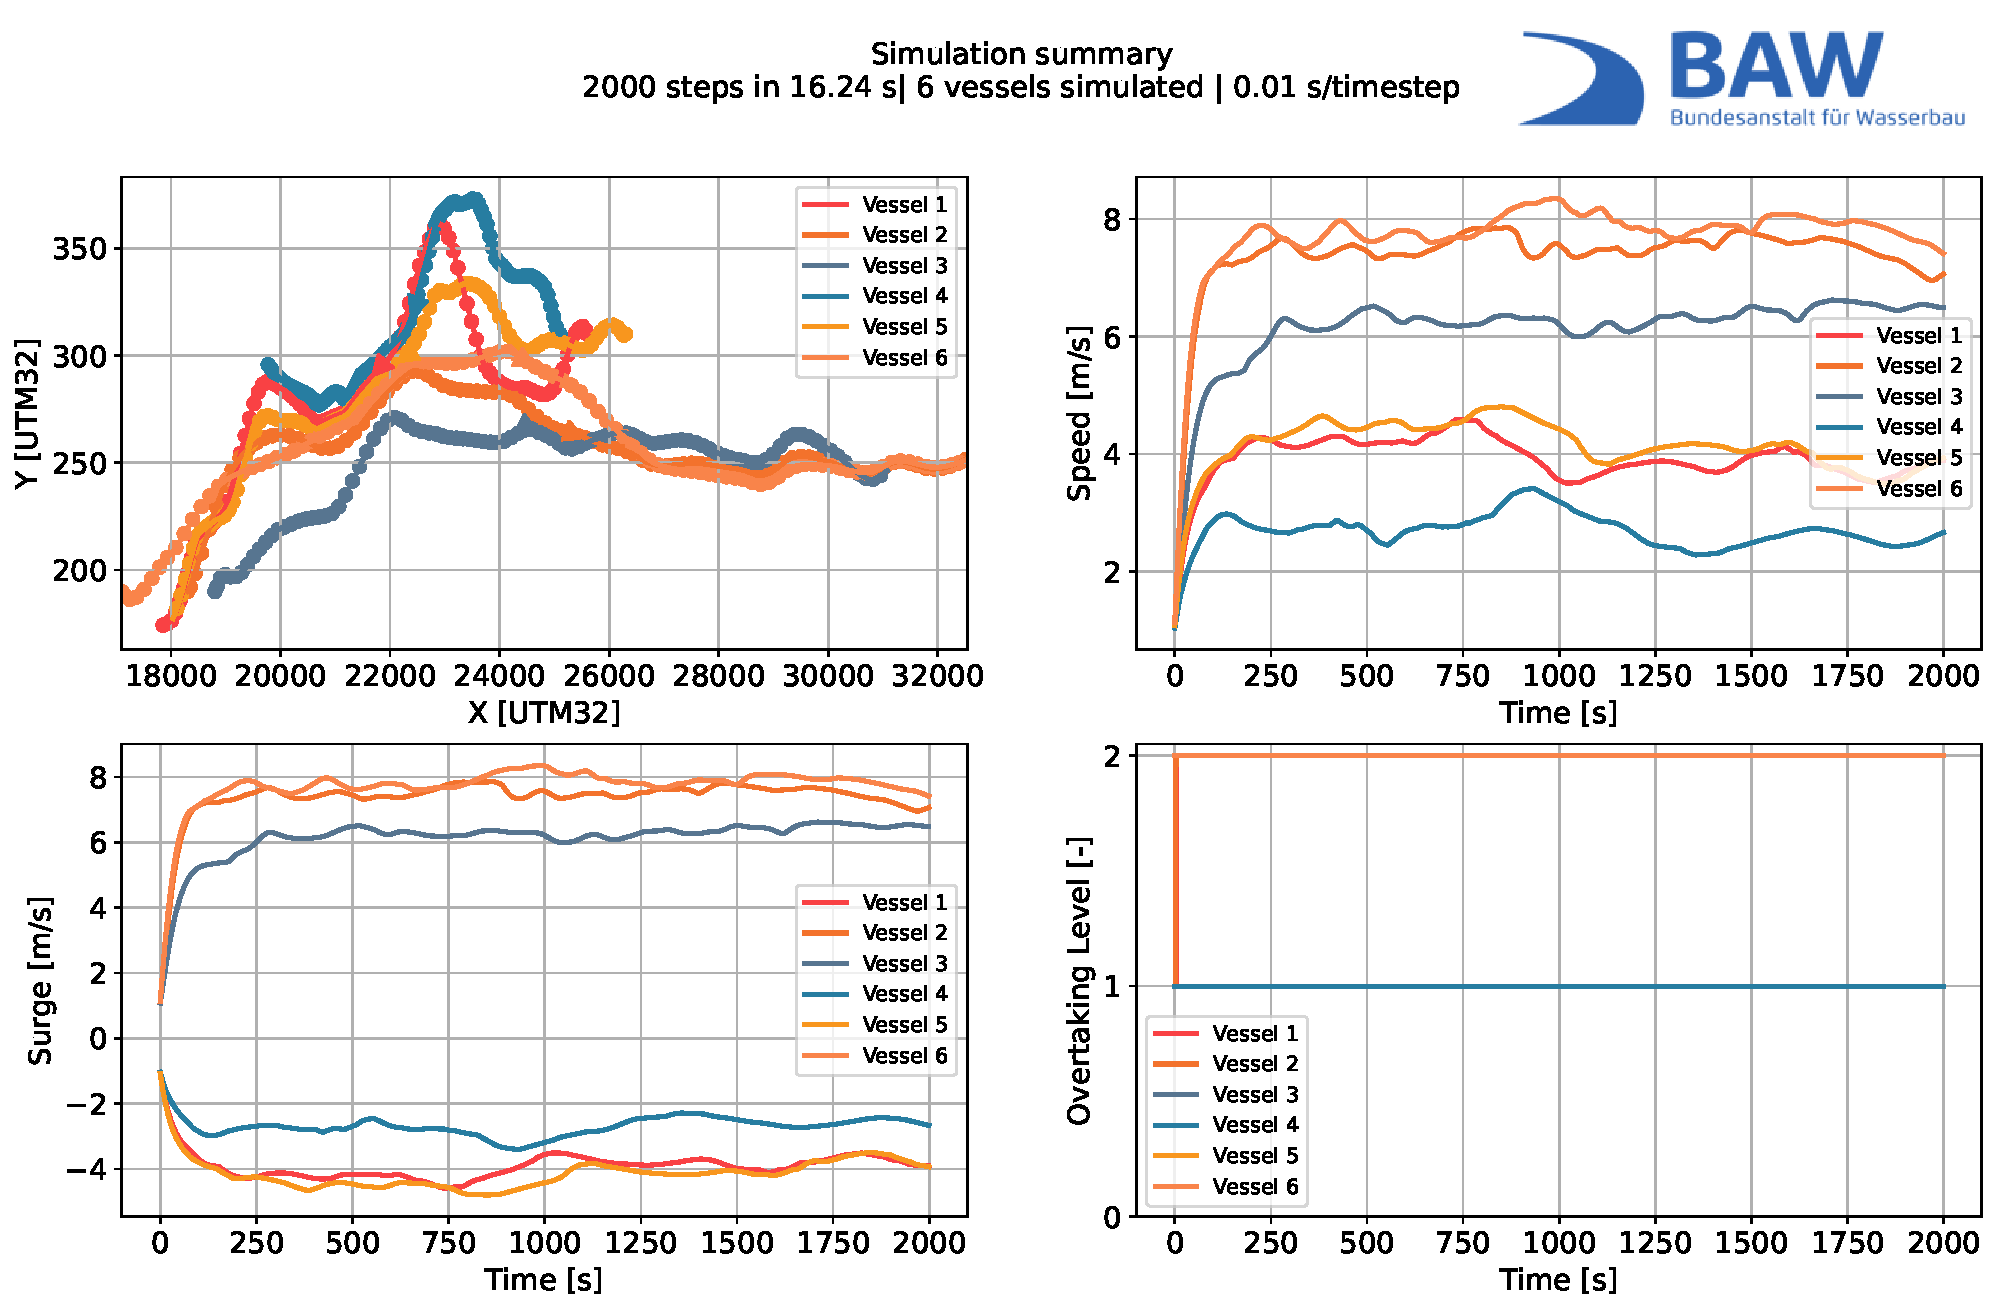
\includegraphics[width=\linewidth]{img/summary.pdf}
	\caption{Graphical logging example.}
	\label{fig:graph}
\end{marginfigure}

We encourage you to adapt the summary plot to your needs. The function is called in the main routine at 

\verb|./src/persist/main.py:129|

and is implemented using the matplotlib library.\sidenote{For example, it may be useful to pass the river object to the summary plotter, so that the river can be plotted in the background alongside the positions of the vessels.}

\subsection{Running PERSIST}

To run PERSIST, simply call it from the command line:

\begin{lstlisting}[language=bash]
	$ persist -c <config_file>
\end{lstlisting}

where \verb|<config_file>| is the path to the configuration file.\sidenote{To avoid file location issues, we recommend to always use absolute paths.}

If you want to run a demo simulation you call call PERSIST with the \verb|--demo| flag:

\begin{lstlisting}[language=bash]
	$ persist --demo
\end{lstlisting}

\begin{note}
	Due to the lack of testing facilites, the calling of PERSIST as a self-contained script could not be tested on Windows machines. If you encounter any problems, please try running PERSIST as a Python module instead. Call it via:
	\begin{lstlisting}[language=bash]
	$ python -m persist -c <config_file>
	\end{lstlisting}
\end{note}

%----------------------------------------------------------------------------------------
%	 REFERENCES/BIBLIOGRAPHY
%----------------------------------------------------------------------------------------

\newpage

\addcontentsline{toc}{section}{Reference List} % Add the bibliography to the table of contents

\begin{twothirdswidth} % Content in this environment to be at two-thirds of the whole page width
	\printbibliography[title=Reference List] % Output the bibliography with a custom section title
\end{twothirdswidth}

%----------------------------------------------------------------------------------------
%	APPENDICES
%----------------------------------------------------------------------------------------

\newpage

\section*{Appendices}

\begin{appendices}

\section{Appendix Section}

Lorem ipsum dolor sit amet, consectetur adipiscing elit. Aliquam auctor mi risus, quis tempor libero hendrerit at. Duis hendrerit placerat quam et semper. Nam ultricies metus vehicula arcu viverra, vel ullamcorper justo elementum. Pellentesque vel mi ac lectus cursus posuere et nec ex. Fusce quis mauris egestas lacus commodo venenatis. Ut at arcu lectus. Donec et urna nunc. Morbi eu nisl cursus sapien eleifend tincidunt quis quis est. Donec ut orci ex. Praesent ligula enim, ullamcorper non lorem a, ultrices volutpat dolor. Nullam at imperdiet urna. Pellentesque nec velit eget euismod pretium.

\section{Appendix Section}

Lorem ipsum dolor sit amet, consectetur adipiscing elit. Aliquam auctor mi risus, quis tempor libero hendrerit at. Duis hendrerit placerat quam et semper. Nam ultricies metus vehicula arcu viverra, vel ullamcorper justo elementum. Pellentesque vel mi ac lectus cursus posuere et nec ex. Fusce quis mauris egestas lacus commodo venenatis. Ut at arcu lectus. Donec et urna nunc. Morbi eu nisl cursus sapien eleifend tincidunt quis quis est. Donec ut orci ex. Praesent ligula enim, ullamcorper non lorem a, ultrices volutpat dolor. Nullam at imperdiet urna. Pellentesque nec velit eget euismod pretium.

\section{Appendix Section}

Lorem ipsum dolor sit amet, consectetur adipiscing elit. Aliquam auctor mi risus, quis tempor libero hendrerit at. Duis hendrerit placerat quam et semper. Nam ultricies metus vehicula arcu viverra, vel ullamcorper justo elementum. Pellentesque vel mi ac lectus cursus posuere et nec ex. Fusce quis mauris egestas lacus commodo venenatis. Ut at arcu lectus. Donec et urna nunc. Morbi eu nisl cursus sapien eleifend tincidunt quis quis est. Donec ut orci ex. Praesent ligula enim, ullamcorper non lorem a, ultrices volutpat dolor. Nullam at imperdiet urna. Pellentesque nec velit eget euismod pretium.

\end{appendices}

%----------------------------------------------------------------------------------------

\end{document}
